%%%%%%%%%%%%%%%%%%%%%%%%%%%%%%%%%%%%%%%%%%%%%%
%       Plantilla Informes Isaias Cardenas
%%%%%%%%%%%%%%%%%%%%%%%%%%%%%%%%%%%%%%%%%%%%%%

\documentclass[letterpaper,12pt]{report}
\usepackage[right=2cm,left=3cm,top=2cm,bottom=2cm,footskip=1.4cm]{geometry}%margenes de la pagina

\usepackage{ucs}
\usepackage[utf8x]{inputenc}
\usepackage[spanish, es-tabla]{babel}
\usepackage[T1]{fontenc}
\usepackage{blindtext}
\usepackage{enumitem}
\usepackage{graphicx}
\usepackage{listings} % escribir codigo
\usepackage{algpseudocode} % escribir algoritmos
\graphicspath{ {./images/} }
\usepackage{multicol} % multicolumnas
% \usepackage{subfigure} % incluir multiples imágenes en una figura
\usepackage{float} % poscicionar imagenes

% \RequirePackage{hyperref}
% \RequirePackage{url} %citacion de URL
% \usepackage{hyperref}
\linespread{1.5} %interlineado

%borra la palabra "capitulo"
\usepackage{titlesec}
\titleformat{\chapter}[display]
    {\normalfont\huge\bfseries}{}{0pt}{\Huge}
\titlespacing*{\chapter}
    {0pt}{10pt}{40pt}

\renewcommand{\contentsname}{Tabla de Contenido}


\begin{document}

\begin{titlepage}

\begin{picture}(0,0)(100,10)
    \put(60,-70){
\includegraphics[scale=0.4]{logo.png}}
\end{picture}

\begin{center}
    \bf{UNIVERSIDAD DE SANTIAGO DE CHILE\\
    FACULTAD DE INGENIERÍA\\
    DEPARTAMENTO DE INGENIERÍA INFORMÁTICA}\\
\end{center}

\begin{center}
    \vspace{4cm}
    \begin{Large}
    \textbf{Entrega 1: Paradigma Imperativo} \\
    \end{Large}
    \vspace{6cm}
\end{center}

\begin{flushright}

\begin{tabular}{lll}
Alumno & : & Isaías Cárdenas A\\
Rut & : & 18750177-6\\
Profesor & : & Luis Celedón\\
Curso & : & Paradigmas de programación\\
Ayudante & : & Christian Vidal\\
% Fecha de entrega & : & 30 de agosto de 2017
\end{tabular}
\end{flushright}
\begin{center}
        \vspace{3cm}
        % Fecha
        \Today
    \end{center}
\end{titlepage}

\tableofcontents
% \listoffigures
% \listoftables

\chapter{Introducci\'on}

\section {Introducci\'on}

El presente documento es la primera entrega de los cuatro proyectos que componen las evaluaciónes del laboratorio para la asignatura Paradigmas de programación, en estos proyectos el alumno debe ser capaz de resolver el problema implementando diferentes lenguajes de programación los cuales a su vez se rigen por distintos paradigmas. Cada laboratorio se enfoca en el mismo problema sin embargo la solución propuesta por parte del alumno debe estructurarse según el paradigma que se trabaje, en este caso se realizará en el paradigma Imperativo utilizando el lenguaje C. Finalmente el alumno manejará completamente el lenguaje C en el paradigma imperativo logrando resolver cualquier problema según éste paradigma.

\chapter{Descripci\'on del problema}

\section {Introducci\'on al problema}

El proyecto consiste en crear un programa que simule un sistema de recuperación de información, similar al que usan los buscadores web en la actualidad. El buscador debe implementar un sistema de indexación para clasificar y ordenar las palabras de diferentes documentos en los que la información será buscada, además de un sistema de ranking que decidirá que documento es mejor resultado que otro en una búsqueda específica. El alumno debe considerar que no todas las palabras formarán parte de la búsqueda, las palabras que deben ser ingnoradas se encontrarán en otro archivo de texto y serán denominadas ``StopWords''. Además se deberá poder guardar un índice invertido en un archivo de texto de manera que el usuario pueda, mas tarde, cargar o leer el mismo indice de modo que no sea necesario leer los documentos nuevamente, simulando consultas a una base de datos. Para implementar éste programa el alumno deberá utilizar el lenguaje de programación C en su versión estándar.

\section {Descripci\'on del problema}

La lectura de los documentos se restringe a la lectura de un archivo de texto que contiene la información de todos los documentos estructurada en el siguiente formato: `` .I '' indica el número que identifica a un documento(id), este indicador es único por lo que no pueden existir dos documentos con el mismo id. `` .T '' es el título del documento, generalmente las primeras 2 líneas que representan al documento. `` .A '' representa a el o los autores el contenido del documento. `` .B '' es un ejemplo de bibliografía para el texto, contiene la información que generalmente solicita el formato APA. `` .W '' es la sección que representa el contenido del texto o documento, puede separarse en párrafos tal como un texto normal. Todos los textos presentes en el archivo de colección de documentos deben contener las secciones descritas y se organizarán en el formato que muestra la figura \ref{fig:ejemploDocsCollections}.


\begin{figure}[H]
    \centering
    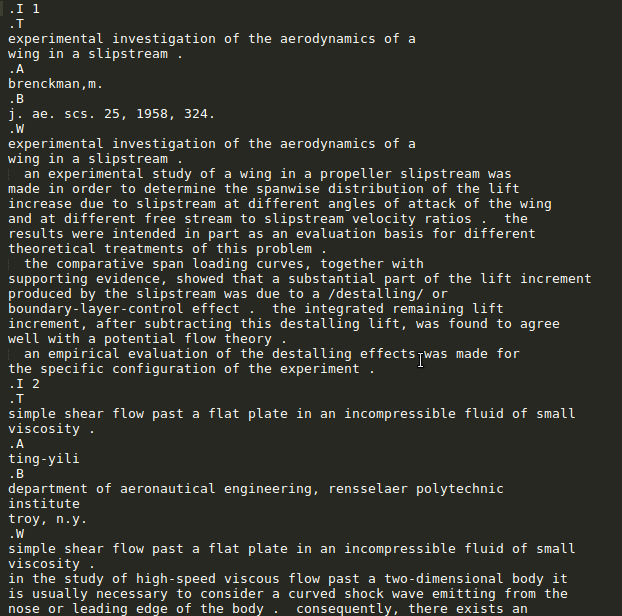
\includegraphics[width=0.4\textwidth]{ejemploDocsCollections.png}
    \caption{Ejemplo de archivo colección de documentos}
    \label{fig:ejemploDocsCollections}
\end{figure}

\vspace{5cm}

Las StopWords estarán en otro archivo de texto que contendrá una palabra por linea, el programa deberá reconocer estas palabras de manera que se ignoren en las frases de búsqueda y a su vez de la lectura de los documentos. la figura \ref{fig:ejemploStopWords} muestra un ejemplo de como debe estar estructurado el archivo de texto con las StopWords.

\begin{figure}[H]
    \centering
    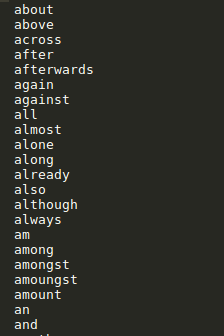
\includegraphics[width=0.4\textwidth]{ejemploStopWords.png}
    \caption{Ejemplo de archivo stop words}
    \label{fig:ejemploStopWords}
\end{figure}

A partir de la lectura de ambos archivos mencionados el alumno debe desarrollar un sistema de indexación implementando un índice invertido o una matriz de incidencia de manera que la información quede estructurada para realizar búsquedas. Esta estructura debe poder almacenarce en un fichero de texto de modo que la información estructurada pueda extrarse sin necesidad de leer los documentos nuevamente (simulando consultas a base de datos). El formato del archivo que contenda la indexación es decisión del alumno.

Con la información organizada el usuario debe ser capaz de realizar consultas al buscador ingresando palabras que serán buscadas en el sistema de indexación y la respuesta serán el conjunto de documentos en los que éstas palabras se encuentran. Los documentos de respuesta deberán ser categorizados según un sitema de ranking que el alumno debe implementar, de modo que un documento será mejor respuesta al usuario que otro según el criterio del sistema de ranking. Además el usuario debe poder solicitar ver los mejores ``k'' resultados a su busqueda, con de ``k'' es la cantidad de documentos respuesta a su busqueda jerarquizados por el sitema de ranking.

Finalmente todas estas funcionalidades debes quedar expresas en un menú donde el usuario podrá elegir la operación que desea realizar. Por otro lado todos los errores y exepciones deben ser controlados mediante el enum descrito en el enunciado de modo que el flujo del programa no se vea interrumpido por entradas inválidas ni errores de segmento. Cabe destacar que el alumno deberá implementar todas las estructuras y funciones descritas en el enunciado entregado por la coordinación de la asignatura sin hacer falta ninguna de ellas.

\chapter{Descripci\'on de la soluci\'on}

Para concretar las funcionalidades para este proyecto, el problema general se subdivide en problemas puntuales mas básicos que en conjunto solucionan y permiten la realización total del proyecto. Para ello se requieren técnicas y herramientas de la informática, en este caso orientadas al lenguaje C, que darán paso a diferentes algoritmos que lograran el correcto funcionamiento del sistema de recuperación de información.

\section {Marco te\'orico}

Para una mejor comprensión de la descripción de la solución es preciso definir algunos conceptos que
serán indispensables en éste proyecto:

\begin{description}[align=left]

\item [Paradigma imperativo:] 
    La programación imperativa es un paradigma de programación que se basa en darle una serie de instrucciones 
    al computador que describan como realizar una tarea, dicho de otro modo, este paradigma busca emular el modo
    imperativo del lenguaje humano. Esta es unos de los primeros paradigmas de programación en consolidarse y al
    igual que en los demás, existen muchos lenguajes de programación que se rigen por este paradigma. La programación
    imperativa es la forma más simple de aprender a programar dado que simula un modo del lenguaje humano de manera que
    no requiere de mucha practica para comprender este paradigma. En este laboratorio se trabajará con el lenguaje C en
    su forma estándar.

\item [Punteros:]
    Los punteros son objetos utilizados en la programaci\'on para referirse o apuntar a algún valor almacenado
    en memoria usando su ubicación, de manera que los valores no necesariamiente deben ser contiguos en memoria.
    El uso de punteros en un lenguaje de programación mejora significativamente el rendimiento de un programa que 
    manipule la información con estructuras de datos (tipos de datos abstractos) y con ello la eficiencia de éste.

\item [Estructura:]
    Una estructura es un conjunto de variables de tipo de datos básico agrupadas en una estructura lógica, esta estructura puede ser utilizada varias veces como un tipo de dato compuesto. El lenguaje C permite la definición de estructuras a fin de facilitar la producción de código al programador.

\item [Lenguaje de programaci\'on ANSI C:]
    El lenguaje C es un lenguaje de programación imperativo estructural caracterizado por
    posibilitar la manipulación de memoria a través de punteros. C es uno de los lenguajes más
    utilizados en el desarrollo de software de sistemas dado que su eficiencia en código es 
    muy alta. El instituto nacional estadounidense de estandarés publicó un estándar para el 
    lenguaje C de manera que a los desarrolladores se les facilitara la portabilidad del código,
    éste estándar fue llamado ANSI C.

\item [Tipos de datos abstractos:]
    Los tipos de datos abstractos o ADT, por sus siglas en el inglés, son tipos de datos complejos u objetos formados a través de estructuras a las que se les ascocian funcionalidades u operaciones. Los ADT se utilizan para estructurar información de manera que la resolución de problemas sea mas organizada facilitando el acceso a los datos que contienen. En general utilizan una interfaz que a través de la cual realiza las operaciones definidas de modo que se abstrae de la forma en que éstas operaciones fueron implementadas. 

\end{description}

\section {Aspectos de implementación}

Para la implementación de este proyecto se utilizaron en general, además de las estructuras y funciones definidas en el enunciado, dos ADT que facilitan el manejo de información en el proyecto:

\begin{description}[align=left]

\item [Listas enlazadas:]
    Las listas enlazadas son un ADT que se forma a partir de nodos conenctados en una dirección utilizando punteros. Cada nodo se encuentra en un lugar diferente en memoria, no nesecariamiente en celdas contiguas, y se accede a través de ellos usando punteros. La absrtacción de la implementación de estos nodos se logra mediante los ``métodos'': get, append, remove, getPosition, isIn, init, etc. Para efecto de la implementación de la solución al proyecto se utilizan dos listas enlazadas, una que contiene enteros(int) y otra que contiene strings (char*).

\item [Tabla hash:] 
    Las tablas hash, también conocidas como contenedor asociativo o diccionario, son una colección de asociaciones de elementos. Relacionan un elemento llave(key) con un contenido(value) de este modo se accede al contenido a través de la llave. Al igual que las listas enlazadas se implementan usando nodos en memoria y se acceden a ellos usando punteros. Tambien se logra la abstracción mediante las funciones: get, append, remove, isIn, init, etc.

\end{description} 

Dicho lo anterior se genera la estructura StopWords utilizando una lista enlazada de strings en la que cada nodo contiene una palabra(stop word). Para generar el índice invertido se implementa una tabla hash en la que cada llave es una palabra, contenida en los documentos, y sus valores son las id's de los documentos a la que cada palabra pertenece, las id's se estructuran en una lista enlazada de enteros; tal y como lo muestra la figura \ref{fig:ejemploIndex}.

\begin{figure}[H]
    \centering
    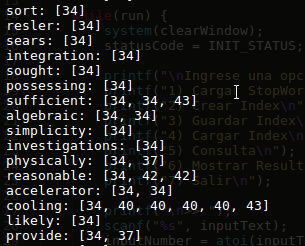
\includegraphics[width=0.4\textwidth]{ejemploIndex.png}
    \caption{Ejemplo de estructura índice invertido}
    \label{fig:ejemploIndex}
\end{figure}

Para organizar los documentos resultados se crea una estructura con los mismos atributos propuestos en el formato de los documentos: id, autores, titulo, bibliografía y contenido; estas estructuras resultado se jerarquizan en una lista enlazada llamada Ranking, de modo que cada nodo contiene un Resultado. Asi para ordenar los resultados por ranking bastará con ordenar la lista enlazada según el puntaje de ranking de cada documento resultado.

\section {Descripción de la solución}

\chapter{Conclusiones}

\section {Conclusiones}

Se cumplen los objetivos propuestos y los requerimientos solicitados en el plazo estipulado, el uso de punteros y el manejo de memoria dinámica se logra en totalidad logarando crear una matriz bidimencional que contiene estructuras. Se observa que tras el manejo de estructuras con punteros las variables se pasan por valor y no por refencia lo que dificultó la implementación de este proyecto; dado que la estructura fue utilizada en varias funciones al intentar cambiar los valores de los atribiutos de éstas las asignaciones solo fueron temporales, es decir, los cambios fueron válidos dentro de las funciones como variables locales. El la próxima entrega se implementarán punteros a estructuras de modo que al utilizar una estructura en una función las variables se pasen por referencia y no por valor, así los cambios no serán temporales.

El uso de varios archivos requiere una organización mas estructurada del proyecto por lo que creó una carpeta llamada ``src/'' en la que se encuentra el código fuente del programa(source), esto provoca que la compilación del proyecto sea mas extensa y tediosa, el uso de un makefile facilitaría la compilación al usuario de modo que en lugar de compilar archivo por archivo lo haga por medio de un solo comando. Esta técnica también favorecería a la ejecución el programa, ya que siempre se realizaría de la misma forma y dependería del alias que le da el usuario al archivo de ejecución.

En sintesis se recomienda utilizar en la proxima entrega: punteros a estructuras para pasos de valores por referencia y makefile para facilitar compilación y ejecución.

\end{document}
